\documentclass{article}
\usepackage[lmargin=2.54cm, rmargin=2.54cm,tmargin=2.54cm,bmargin=2.54cm]{geometry}
\usepackage{doc}
\usepackage{graphicx}
\usepackage{indentfirst}
\usepackage{setspace}
\doublespacing

\title{Microsoft Word Added Dream Interface}
\author{Anthony Menjivar}

\date{12/6/13}

\begin{document}

\maketitle

\abstract{
	This dream design document contains a made up interface using an already established system and how it would seen in interaction design terms as in why and how it was made up for that system. The specific system used for this dream interface will be Microsoft Word (2013). The tool/interface from the made up dream design will be specifically for Microsoft Word but can be used in other Microsoft systems. This tool can be seen as an idea from other interfaces already seen in the world of software but will be given specific and new detail as to how it will be used in the Word Processor and why it can be useful in Microsoft Word.
} % JD: Ah, a word processor dream interface.  This can be interesting.

\section{Introduction}	
\indent	The Microsoft Word processor has been around since the 1980s and since then has been brought up to have the many useful features that it has. Nowadays it can be seen in the Microsoft Office software, which also contains other big programs such as Microsoft Excel and Microsoft PowerPoint, just to name a few, and has become a big and important software in today's world, especially in the life of students, even though it doesn't stop at school. As just said, the word processor contains many features and has gained more and more as the years have gone by and has all the really neat features that it has today in it's current version, Microsoft Word 2013. A couple features we see in the newest version of the word processor include being able to convert PDF files into word documents, connecting online with other devices that use the processor and seeing what was last recently worked on, new templates for the documents and also just a new layout from what it looked like in previous versions. All in all, Word keeps being developed and grown to accommodate as much as it possibly can as well as make it the easiest and fastest word processors for users to experience.	

	With the thought of easiness and quickness coming up for Microsoft Word, there may still be new features or tools that may come up for the software to have for users to experience. This is where the dream design interface that this document will discuss comes into play as the idea of it and it's features of how it would work came from a perspective of bringing easiness and quickness for the user to accomplish a task that may be common in many people using Microsoft Word.
% JD: Remember, for "it_s," you only use an apostrophe if the word is a
%     contraction for "it is."  In all other cases, *no* apostrophe.

	The tool interface for this dream design that would be implemented to Microsoft Word will be given the name Para-Snip. The name goes along, in a way, with what the tool does in the Microsoft Word processor. This tool should be an interface that comes in handy when users are writing essays, reports or things of that nature that contain multiple paragraphs. This tool will be displayed as a designed button and will be added to the Word processor's toolbar. When a word document has paragraphs and the button is clicked on, the Para-Snip interface will separate the essay into all the paragraphs in which it contains and let the user move around the paragraphs however they like to restructure the document. Para-Snip is a tool that would be used very often in the Microsoft Word program when it comes to editing essays or reports after users are done with the document that they are working on. In this Dream Design document I will go into full detail on how the Para-Snip will work and go in to the Interaction Design parts of the usage of the tool with the Word processor.
% JD: This actually does not sound very different from Word's Outline
%     mode.  I hope that you are able to show the distinction...

\section{Para-Snip}

\subsection{Description}
	The idea of the Para-Snip came from being student myself and looking at tools that would be very handy for when I do work, specifically essays, which every student has to go through no matter what it is they may be doing. When I thought about editing papers, I thought about how there are various times where you look back at the paper and realize some paragraphs may not fit where you want them and in general it would be better to move ideas around. Also the user may also just want to see how the paper flows having different ideas in different areas of the paper. With this tool, the user can perform all of that.

	When the Para-Snip button on Microsoft Word is clicked, the document will go into a mode where the paragraphs are emphasized and separated within the document. Each paragraph then can be labeled in any way in order for the user to know what each paragraph is. The user will be able to drag and drop  paragraphs in between other paragraphs while also having a column on the side where paragraphs can be dropped to hold until they are placed back or in another location in the paper. The main goal behind this Para-Snip tool is to bring efficiency and easiness to the user when trying to restructure papers or reports to come out the best way possible. We will go into the layout of how this tool will be seen and more detail on how it can/will be used.
% JD: OK, good, I see some distinction here.  But you should still
%     acknowledge the potential similarities with Outline mode.

\subsubsection{Touch-Screen}
	A quick side note on the description of this tool that would be very useful and could go best with a touch screen device as well. This tool will have a drag and drop feature when it comes to moving around paragraphs in the document. A touch screen device would allow the user to literally grad hold of the paragraph and either place in the paragraph holders on the side column or anywhere within the document. This will give the tool the best hands on feel to it and could be very interactive to the user making it even easier for the user to use.
	
\subsection{Layout}
	Here we will go into full detail on how the Para-snip will look in Microsoft Word and use images to give an idea of what the user will be looking at when using this tool.

% JD: Great, thank you for providing illustrations.
\begin{center}
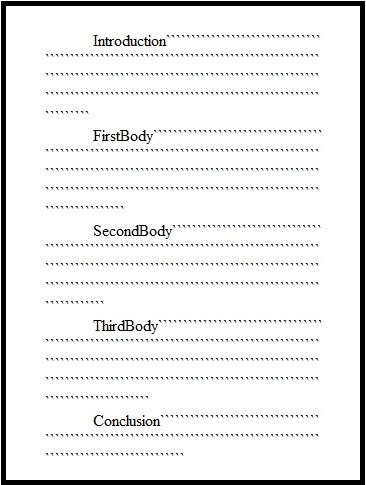
\includegraphics[width=60mm]{BeginEssay.jpg}
\end{center}
\begin{center}
Image 1: Sample Essay Document
\end{center}
	
	We see many people use Microsoft Word to create documents for school, work or even for personal reasons. In image one, we see a picture of a document that we will say is an essay with five paragraphs (introduction, three body, and conclusion) created on Microsoft Word. We will use these five paragraphs in this document to show how the Para-Snip will be used. The document will be seen in the general stages of what will happen when using the tool.
	
\begin{center}
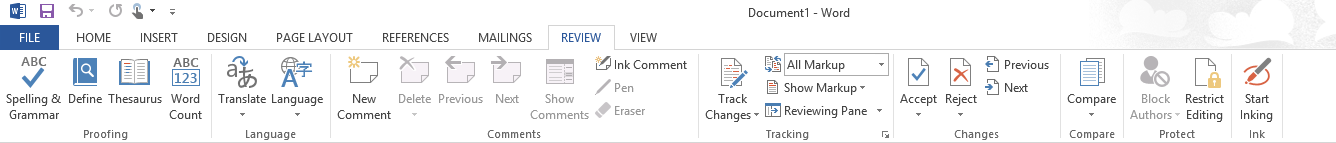
\includegraphics[width=150mm]{MWReview.png}
\end{center}
\begin{center}
Image 2: Microsoft Word Review Tab
\end{center}
\medskip

	Microsoft Word will have a new button called the Para-Snip button in the toolbar. Microsoft Word does have tabs for different tools on the top of documents so the best option would be to put this button under the review tab, as seen in image 2, since the tool is used to review and restructure documents after they paragraphs have been made. It could go in a new section called paragraph since the paragraphs are the main part being edited with this tool.
\bigskip

\begin{center}
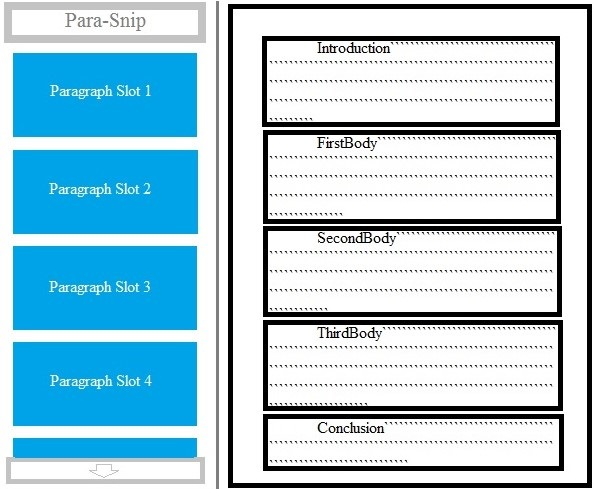
\includegraphics[width=100mm]{Essay2.jpg}
\end{center}
\begin{center}
Image 3: Design of Para-Snip Mode in Microsoft
\end{center}
\medskip

	When the Para-snip button under the Review tab is licked on, the document will go into a paragraph editing mode as seen in image 3. The mode will bring up a column on the left-hand side of the document with the actual Para-Snip tool, containing slots to place paragraphs from the document in them. The empty slots will be a light colored blue to go along with the color theme of Microsoft Word and not make it too different. The document itself will also be changed a little in the Para-Snip mode. All the paragraphs in the document will get a separation box around them in order to be able to drag and drop paragraphs as the user pleases. Paragraphs will be given the option of being named to let the user know which paragraph is which.
	
\begin{center}
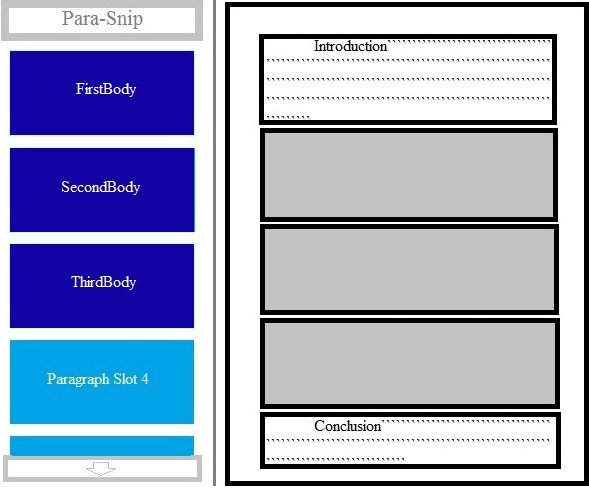
\includegraphics[width=100mm]{Essay3.jpg}
\end{center}
\begin{center}
Image 4: Example of Para-Snip Editing
\end{center}
\medskip

	Image 4 contains the mode with paragraphs being moved into the slots. These paragraphs were drag and dropped by the user from the document into the paragraph slots. The slots that already contain a paragraph in them will be denoted by a darker blue color so the user knows to use a different slot if they choose to drop another paragraph in one of the slots. When paragraphs are removed from the document, there will be empty slots in the document which will be denoted by gray boxes within the document. This is where those paragraphs in the slots or other paragraphs in the document can be placed. 
% JD: Although there are differences from Outline mode, they are somewhat
%     subtle.  Plus, what you are doing is also not that different from
%     just selecting an entire paragraph (triple-click) then doing drag-and-drop
%     on it.  Similarities are OK, but it is better to point them out clearly,
%     so that you can emphasize what's different or better.

\begin{center}
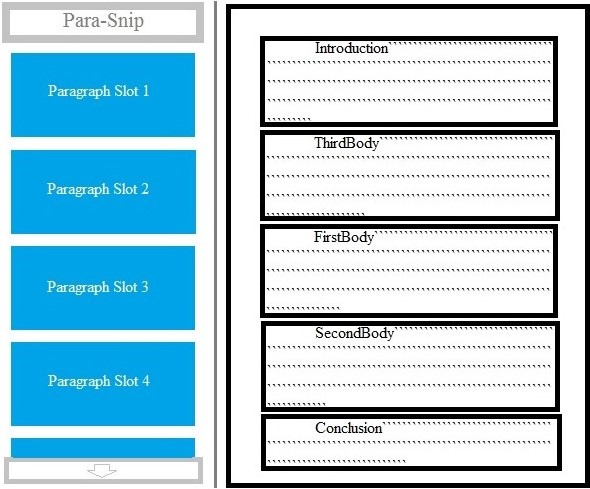
\includegraphics[width=100mm]{Essay4.jpg}
\end{center}
\begin{center}
Image 5: Example of Final Para-Snip Editing
\end{center}
\medskip

	The paragraphs can be moved around in many ways and as the user pleases to get to the user's preferred structure. Image 5 shows a small sample of how a document would look after paragraphs have been restructured to the user's wanting. In order to finish the Para-Snip button is to be pressed again and the document layout would go back to normal  for regular editing of the paper. If the document had been saved before, the document will be automatically saved once the button is pressed to exit the Para-Snip mode so the user doesn't have to do it.
% JD: OK, I was wondering about this.  So all changes stay in the Para-Snip
%     area until the user dismisses it.  Not quite as immediate as drag-and-drop,
%     I guess, but I can see how that can work.

	There are layout features that are not really seen in the images. There is the being able to scroll up and down the empty paragraph slots on the side since plenty of paragraphs can be placed in slots that they all wouldn't be able to fit in the screen. There is being able to move the paragraphs within the document and not necessarily having to put paragraphs in the empty slots. Moving a paragraph above or below another paragraph would move that next paragraph to where the previous paragraph was. Smaller features it contains would include things such as an undo button, a redo button, a delete button and an add button, in case empty space wants to be left for the user to add more in between certain paragraphs but doesn't want to leave the Para-Snip tool yet. 
% JD: Now *this* part *really* sounds like drag-and-drop.

	These are little features along with the main part of the tools interface that will make up the Para-Snip tool in its entirety and how it would be used.
	
\subsection{Usage Scenarios}

	One example of where the Para-Snip can be used can be within the usage of Microsoft Word from a college Student. College Students are writing essays all the time for their classes and editing is a very tedious thing to do for them. The Para-Snip tool can make it a bit easier and quicker for the editing. Sometimes when students write papers, after they are done, they may realize they said somethings first when they wanted to say something else first or they just wonder if the essay would have better flow if ideas in certain paragraphs were switched around. The Para-Snip tool will allow them to switch around paragraphs to read how the flow of the essay would be and let them place wherever they may want the paragraphs to be. This is definitely a case in which the tool will come in handy, making it more efficient on the student working on the essay.
	
	Another example could be in reports done for a job. Jobs always look for perfection in reports and any documents. Because of this, editing is a huge part in order to make the report perfect to turn in. Same as the college student, editing can be very tedious and even sometimes frustrating if you are looking for perfection. The Para-snip tool can help ease the frustration of editing paragraphs and the flow of reports as to see which way makes the best report to turn in. 

\section{Interaction Design View}

\subsection{Rationale}
	There are many reasons of behind the coming up of the idea of the Para-Snip. As has been brought up before, Microsoft Word is always being being developed to not only make it look good but also to make the software easier and more efficient for users. The Para-Snip tool would fit in greatly with the development of Microsoft Word and can be seen as a very useful addition.
	
	We first look at the proposed layout of the Para-Snip tool along with the layout of the Microsoft Word program in general. Microsoft Word already has a good looking layout that is very pleasing to the eye and really it can sometimes be a reason why users like it. The Para-Snip tool will have a layout that will fit in to the layout of the program itself. This is to ensure consistency within the program and the tool. Therefore colors and the way the tool is shaped in comparison to the document will go along with the how the colors and shapes look in the program. Consistency within a program is big especially when it comes to viewing a program and this will make it pleasing to the eye of the user.
	
	This small interface will also have the universal features such as undo redo. This also keeps it consistent with the program itself as this interface is meant to be as consistent as possible with Microsoft Word.
	
	We go onto human interaction with the Para-Snippet tool. When it comes to features of programs in software, one of the best things to have would be to have real life like features to it (in a way seen in the use of touch screen). The drag and drop feature that this tool contains makes the user feel like they are actually moving around objects and is a lot better than just clicking on buttons to make something happen. This interaction makes a task easier to follow in an event as they know what is happening the whole way through. This can be seen as direct manipulation within the Para-Snip interface and is best for the visual part while it is being used.
	
	Other small features would be having visual aids within the Para-Snip tool. These small features range from having names on things such as on the paragraph slots or showing that you could scroll down the slots column. Then there are having boxes to emphasize the paragraphs along with the colors of the boxes and slots; different colors show where there is an empty slot or a filled slot. Even the smallest features such as these make the interface much better for the user and they will definitely be taken into account for the Para-Snip tool.	
% JD: The notion of drag-and-drop is easy to invoke on paper, but it has
%     some implications.  For example, if I drag a paragraph from its
%     original slot and drop it over a new slot, what happens to the paragraph
%     that was in that slot?  Does it:
%
%     - get erased?
%     - exchange places with the original paragraph? or
%     - does the dragged paragraph get inserted either before or after the
%       dropped area?
%
%     Notice how this answer is not obvious.  It may have been obvious to you
%     because the paper does not address it, but believe me it is not obvious
%     to the reader...and thus, it will also not be obvious to the user.

\subsection{Usability}
	When talking about usability metrics for the Para-Snip tool we will talk about five metrics: Learnability, Efficiency, Memorability, Errors, and Satisfaction. Since the tool interface has not been created yet but what we will be talking about here will be how the Para-Snip tool would fall under each of these categories were it to actually exist in Microsoft Word and tried out. The discussion, using the five usability metrics will be in a general light.

\subsubsection{Learnability}
	When it comes to learnability the Para-Snip tool can vary. This is because the knowledge of the Microsoft Word processor can vary also. If users have no knowledge of Microsoft Word it will obviously take that much longer for a user to learn it as the user will have to learn the word processor first. But if the user has knowledge of the word processor then the user wouldn't take to long to learn to use the tool. The Para-Snip tool is pretty self explanatory and interactive enough, with the drag and drop feature, for the user to learn how to use it for the document.
% JD: You're sort of begging the question here.  What specific elements or
%     characteristics foster learnability?  These are not identified; you
%     just say it's self-explanatory without saying what *makes* it self-
%     explanatory.
	
\subsubsection{Efficiency} 
	For efficiency, I decided to compare using the Para-Snip tool with just the regular old copy and paste or drag feature already in the word processor. Without actual numbers, The Para-Snip tool would be best if a user has to keep moving around paragraphs as they please and will help the user go that much faster with finishing the document. This is better than going back and forth with the other features it has.
% JD: OK, this is a little better.  But I think you miss the key differentiator,
%     which is that, using normal drag-and-drop, it takes a little more time to
%     select whole paragraphs then precisely position them (because regular
%     drag-and-drop allows the user to drop a paragraph *inside* another one).
%     So it simply takes more maneuvering.

\subsubsection{Memorability} 
	With the interactive style of Para-Snip, the tool seems like it would be very easy to remember. Interactivity means the user is more likely to remember it and the drag and drop feature adds that to the Para-Snip tool.
% JD: "Interactivity" in this context does not really have a meaning.  Memorability
%     is a given if the system is highly learnable.  So, if you make that case, then
%     you actually don't have to worry about memorability.

\subsubsection{Errors} 
	Errors is a hard thing to see when we can't actually test the tool if it hasn't been made. In general, obviously more errors would be made if a user has no experience of Microsoft Word. In this case errors would be made even if they don't have to do exactly with the Para-Snip tool as they try and look for it. As for experienced user. The Para-Snip tool, from its description seems to be an editing tool and therefore it would be thought to be contained under the review tab in the toolbar. Even in the case of errors, when it comes to editing with the Para-Snip, the user may have to be moving paragraphs back and forth to their liking and errors may not actually play a big part with this tool, at least when it comes to human error.
% JD: On the contrary, I think you can certainly identify potential errors without
%     having to implement the interface.  To name a couple:
%
%     - User can pick the wrong paragraph to drag
%     - User can drop the paragraph in the wrong location
%
%     You don't need to implement the tool to see those possibilities, nor do you
%     need to implement the tool to come up with ways to minimize those errors.

\subsubsection{Satisfaction} 
	Yes, this tool is only a small interface to the big program of Microsoft Word. But when it comes to those frustrating times of editing with Microsoft word, this tool can be very useful and pleasing to the user but satisfaction levels can vary greatly from users that will use it very often to those that may not use it at all.
% JD: Yes, this one really is a tough one to call, especially for a utilitarian
%     application like Word.  I don't think you even need to address it here.

\section{Conclusion}
	The Para-Snip tool would be a great tool to see in the Microsoft Word software. It can be a very useful tool to the work of many as Microsoft Word is such a huge program in the world of technology in today's world. The word processor always seems to make improvements as it comes out with new versions and this could be a great dream addition to it. The Para-Snip tool could bring much needed efficiency to working on documents and would fit in with the use of Microsoft Word for a lot of documents.
% JD: You didn't follow up on a feature mentioned early on that I actually think
%     makes Para-Snip more distinct from Outline or drag-and-drop: the labeling of
%     paragraphs.  At the beginning you said that this is one of the capabilities
%     or Para-Snip, but it was never detailed further.

\end{document}
